% Example LaTeX document for GP111 - note % sign indicates a comment
\documentclass[12pt,a4paper,oneside]{article}
\usepackage{lmodern}
\usepackage[french]{babel}
\usepackage[T1]{fontenc}
\usepackage[utf8]{inputenc}
\usepackage{graphicx}
\usepackage{hyperref}
\usepackage{float}


% Default margins are too wide all the way around. I reset them here
\setlength{\topmargin}{-.5in}
\setlength{\textheight}{9in}
\setlength{\oddsidemargin}{.125in}
\setlength{\textwidth}{6.25in}

\hypersetup{
    unicode=false,          % non-Latin characters in Acrobat’s bookmarks
    pdftoolbar=true,        % show Acrobat’s toolbar?
    pdfmenubar=true,        % show Acrobat’s menu?
    pdffitwindow=false,     % window fit to page when opened
    pdfnewwindow=true,      % links in new window
    colorlinks=true,       % false: boxed links; true: colored links
    linkcolor=black,          % color of internal links (change box color with linkbordercolor)
    citecolor=green,        % color of links to bibliography
    filecolor=magenta,      % color of file links
    urlcolor=cyan,          % color of external links
    linktoc=page
}

\begin{document}
\title{\textbf{\Huge{Rapport SIG}}}
\author{
	\textit{Jordan FONTORBE}\\
	\textit{Willy FRANÇOIS}\\
	\textit{Jérémy MOROSI}\\
	\textit{Jean-Baptiste PERRIN}
}

\maketitle
\newpage

\tableofcontents
\newpage

\section{Introduction}


\section{Analyse}

\subsection{Architecture}
% diagrammes
% intéractions


\section{Réalisation}

\subsection{Commun}
\subsubsection{Package geometry}
\subsubsection{Package data}
Le package \textbf{data} contient le modèle des données ainsi que les fonctions (SQL et XML) nécessaire au prétraitement des données.
\paragraph{Le modèle : \\}
Notre modèle correspond à la structure de notre base de données. Nous avons choisi de ne garder que les nœuds, les trous, les routes, les bâtiments, les bassins et les forêts. Ainsi nous retrouvons : \\
\renewcommand{\labelitemi}{$\bullet$}
\begin{itemize}
\item une classe \textbf{Node} contenant un \textit{id}, une \textit{latitude} et une \textit{longitude}. Cette classe caractérise un point de la carte et va permettre avec ses coordonnées de construire une route, un bâtiment, un bassin ou une forêt.
\item une classe \textbf{Road} contenant un \textit{id}, un \textit{nom} (pas obligatoire),  un \textit{type} (route secondaire, chemin, route piétonne, etc.), la liste des nœuds qui la constitue et sa \textit{géométrie}.
\item une classe abstraite \textbf{Structure} possédant un \textit{id}, un {nom} (pas obligatoire), la liste des nœuds qui constitue cette structure, sa géométrie ainsi que la liste de ses trous (peut être vide). Les classes héritant de \textbf{Structure} sont :
	\begin{itemize}
	\item la classe \textbf{Building}. Elle représente un bâtiment et à en plus une liste de tous ses nœuds proches (hors ceux constituant le bâtiment).
	\item la classe \textbf{Basin} décrivant un bassin (lac, étang, etc.)
	\item la classe \textbf{Forest} décrivant une forêt.
	\item la classe \textbf{Hole} décrivant un trou d'une structure. Elle possède en plus l'id de la structure à laquelle il appartient.
	\end{itemize}
\end{itemize}
Le modèle est représenté par le schéma ci-dessous :\\

\begin{figure}[H]
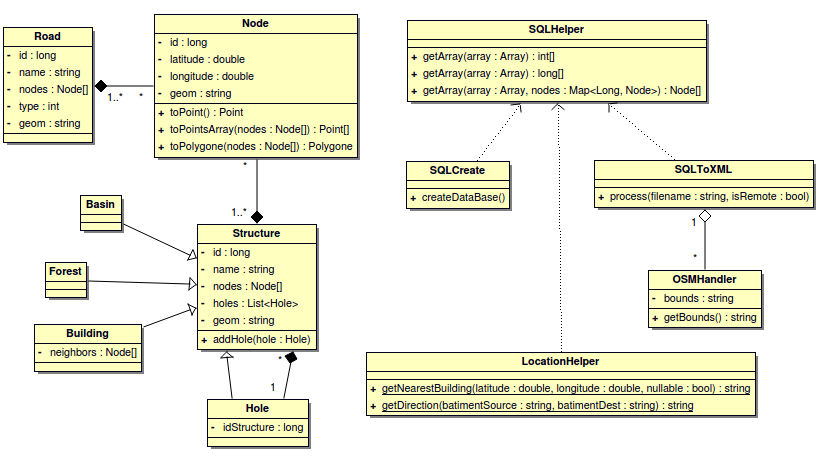
\includegraphics[width=1\textwidth]{../images/modeleDonnees.png}
\caption{Modèle}
\end{figure}

\paragraph{Le pré-traitement : \\}
Une étape de pré-traitement à été nécessaire. En effet lorsque nous avons récupérer les données \textit{OpenStreetMap} et importé dans une base de données (à l'aide de l'outil \textit{osm2pgsql}), nous avons dû récupérer seulement les informations qui nous étaient utiles. Ainsi nous avons créé 4 nouvelles tables correspondant à notre modèle (sig1337\_nodes, sig1337\_roads, sig1337\_holes et sig1337\_structures) avec seulement les informations nécessaire (coordonnées, géométrie, nom, ...). Cette génération se fait à l'aide de la classe \textbf{SQLCreate} du package \textbf{data.sql}. \\
Ensuite, les données vont être récupérées et parsée en XML. On retrouvera notamment les tags :
\begin{itemize}
\item \textbf{bassin}, contenant un nom, une liste de voisins, et les triangles permettant sa construction en \textit{OpenGL}.
\item \textbf{foret}, contenant un nom, une liste de voisins, et les triangles permettant sa construction en \textit{OpenGL}.
\item \textbf{batiment}, contenant un nom, une liste de voisins, et les triangles permettant sa construction en \textit{OpenGL}.
\item \textbf{route}, contenant la liste des points la décrivant et son type (chemin ou route pour une réprésentation différent sur la carte).
\end{itemize}

\newpage

\subsection{WebService}
Afin de permettre une utilisation de l'application en mode "remote", un \textit{WebService} a été mis en place. Aucune donnée (comme les bâtiments, les routes, l'arbre de décision) n'étant stockée sur le téléphone dans ce mode, c'est l'appel aux méthodes de ce \textit{WebService} qui va nous permettre de récupérer toutes les données nécessaires. \\
Il permet entre autre d'avoir accès à trois méthodes :\\
\begin{itemize}
\item Une méthode permettant de récupérer les informations de la carte au format XML, c'est-à-dire les nœuds, les routes et les structures ainsi que l'arbre de décision. Cette méthode sera appelée au lancement de l'application en mode "remote". Elle est accessible à partir de l'URL : http://\textit{IP\_ADRESS}:\textit{PORT}/WebService/service/map. La définition de cette méthode est présente dans la classe \textbf{MapService}.
\item Une méthode permettant à partir d'une latitude et d'une longitude, de récupérer le plus proche bâtiment. Elle sera appelée dans l'application Android, lors d'un appuie sur une zone de la carte afin de pouvoir sélectionner un bâtiment comme point de départ ou d'arrivée pour un itinéraire. Cette méthode est accessible à partir de l'URL : http://\textit{IP\_ADRESS}:\textit{PORT}/WebService/service/location/building/\{lat\}/\{lon\}. Elle est définie dans la classe \textbf{LocationService}.
\item Une méthode permettant à partir de l'identifiant d'un bâtiment de départ et de l'identifiant d'un bâtiment d'arrivée de retourner un itinéraire (au format JSON). La réponse renvoie la liste des coordonnées à parcourir. Cette méthode sera appelée lors de la demande de calcul d'un itinéraire par l'utilisateur et est accessible à partir de l'URL : http://\textit{IP\_ADRESS}:\textit{PORT}/WebService/service/location/direction/\{id départ\}/\{id arrivée\}. Cette méthode est définie dans la classe \textbf{LocationService}.\\
\end{itemize}

La méthode récupérant le XML décrivant la carte étant la plus longue, c'est un tâche asynchrone qui l'appel. Les deux autres méthodes étant relativement rapide (une seconde environ), on attend la réponse du WebService (avec une limite fixée à 3 secondes pour ne pas bloquer l'application trop longtemps). 

\newpage

\subsection{Android}
\subsubsection{Version locale}
\subsubsection{Version distante}


\section{Difficultés rencontrées}


\section{Répartition du travail}


\section{Conclusion}


\appendix
\end{document}
